\documentclass{article}

%Headers
\usepackage[dvips]{graphicx}    %package that does pdfs
\usepackage{color}              %this needs to be here also
\usepackage[T2A]{fontenc}
\usepackage[utf8]{inputenc}
\usepackage{listings}

\lstdefinestyle{pythonstyle}{
  language=Python,
  basicstyle=\small\ttfamily,
  keywordstyle=\color{blue},
  commentstyle=\color{green},
  stringstyle=\color{black},
  showstringspaces=false,
  tabsize=4,
  frame=single,
  numbers=left,
  numberstyle=\tiny\color{black},
  stepnumber=1,
  numbersep=8pt,
  firstnumber=1,
  breaklines=true,
  xleftmargin=15pt,
  framexleftmargin=15pt,
  backgroundcolor=\color{white},
  captionpos=b
}



\title{Практическая работа по дисциплине "Нейроэволюционные вычисления"}
\author{Малкин Артем студент гр. 8ВМ22 НИ ТПУ}

\date{19 Мая 2023}

\begin{document}
\maketitle


%Note that the '*' surpresses the section numbering
\section*{Номенклатура}
\label{sec:nomenclature}
\begin{tabbing}
    XXXXXXXX \= \kill% this line sets tab stop
	NEAT				\> NeuroEvolution of Augmenting Topology\\    
	CUDA 				\> Compute Unified Device Architecture	
\end{tabbing}

\section{Постановка задачи}
Эта секция описывает задачи, поставленные в рамках практической работы.

\subsection{Программный код}
В рамках практической работы был разработан программный код с применением модуля PyTorch для реализации нейроэволюционного алгоритма NEAT. Программный код был разработан на языке Python.

% add program code abd color it
\begin{lstlisting}[style=pythonstyle, caption={Программный код реализации алгоритма NEAT с применением модуля PyTorch}, label={lst:pythoncode}]
	import torch
	import torch.nn as nn
	import torch.optim as optim
	from torchvision.datasets import MNIST
	from torch.utils.data import DataLoader
	from torchvision.transforms import ToTensor
	import neat
	
	# Define the PyTorch-based neural network class
	class NeuralNetwork(nn.Module):
		def __init__(self, input_size, output_size):
			super(NeuralNetwork, self).__init__()
			self.fc = nn.Linear(input_size, 64)
			self.relu = nn.ReLU()
			self.out = nn.Linear(64, output_size)
	
		def forward(self, x):
			x = self.fc(x)
			x = self.relu(x)
			x = self.out(x)
			return x
	
	# Define the fitness evaluation function
	def eval_fitness(genomes, config):
		for genome_id, genome in genomes:
			net = neat.nn.FeedForwardNetwork.create(genome, config)
			criterion = nn.CrossEntropyLoss()
			optimizer = optim.Adam(net.parameters(), lr=0.01)
			for batch_images, batch_labels in train_loader:
				batch_images = batch_images.cuda()
				batch_labels = batch_labels.cuda()
	
				optimizer.zero_grad()
				outputs = net.activate(batch_images.view(batch_images.size(0), -1))
				loss = criterion(outputs, batch_labels)
				loss.backward()
				optimizer.step()
			
			# Evaluate the fitness
			correct = 0
			total = 0
			for test_images, test_labels in test_loader:
				test_images = test_images.cuda()
				test_labels = test_labels.cuda()
				
				outputs = net.activate(test_images.view(test_images.size(0), -1))
				_, predicted = torch.max(outputs.data, 1)
				total += test_labels.size(0)
				correct += (predicted == test_labels).sum().item()
			
			accuracy = correct / total
			genome.fitness = accuracy
	
	# Load MNIST dataset
	train_dataset = MNIST(root='./data', train=True, transform=ToTensor(), download=True)
	train_loader = DataLoader(train_dataset, batch_size=32, shuffle=True)
	test_dataset = MNIST(root='./data', train=False, transform=ToTensor(), download=True)
	test_loader = DataLoader(test_dataset, batch_size=32, shuffle=False)
	
	# Configure NEAT
	config_path = 'neat-config-file.cfg'  # Specify the path to your NEAT configuration file
	config = neat.config.Config(neat.DefaultGenome, neat.DefaultReproduction, neat.DefaultSpeciesSet,
								neat.DefaultStagnation, config_path)
	
	# Create the population
	population = neat.Population(config)
	
	# Add a reporter to display the progress during evolution
	reporter = neat.StdOutReporter(True)
	population.add_reporter(reporter)
	
	# Run NEAT
	best_genome = population.run(eval_fitness, 100)
	
	# Retrieve the best neural network from the evolved population
	best_net = neat.nn.FeedForwardNetwork.create(best_genome, config)
	
	# Test the best neural network
	with torch.no_grad():
		correct = 0
		total = 0
		for test_images, test_labels in test_loader:
			test_images = test_images.cuda()
			test_labels = test_labels.cuda()
			
			outputs = best_net.activate(test_images.view(test_images.size(0), -1))
			_, predicted = torch.max(outputs.data, 1)
			total += test_labels.size(0)
			correct += (predicted == test_labels).sum().item()
		
		accuracy = correct / total
		print("Accuracy of the best network: {:.2f}%".format(accuracy * 100))
\end{lstlisting}

\subsection{ВСЁ, что ниже, (и таблица выше) - не моё, а fake-информация, не относящаяся к NEAT}
The goals of this experiment are as follows:

%Illustrate using a list
\begin{itemize}
    \item Flight test a small unmanned aerial system (UAS).
    \item Demonstrate viability of using an aviation tranponder onboard a UAS.
\end{itemize}

The aircraft used in the experiment is shown in Figure~\ref{fig:Aircraft}.  This was flight tested on several occasions \cite{Lum_ADSB_sUAS_2017} and uses autonomous algorithms to perform search and rescue \cite{Lum_Searching_JACIC_2010}.  

%Illustrate inserting a figure
\begin{figure}[ht]
	\centering
    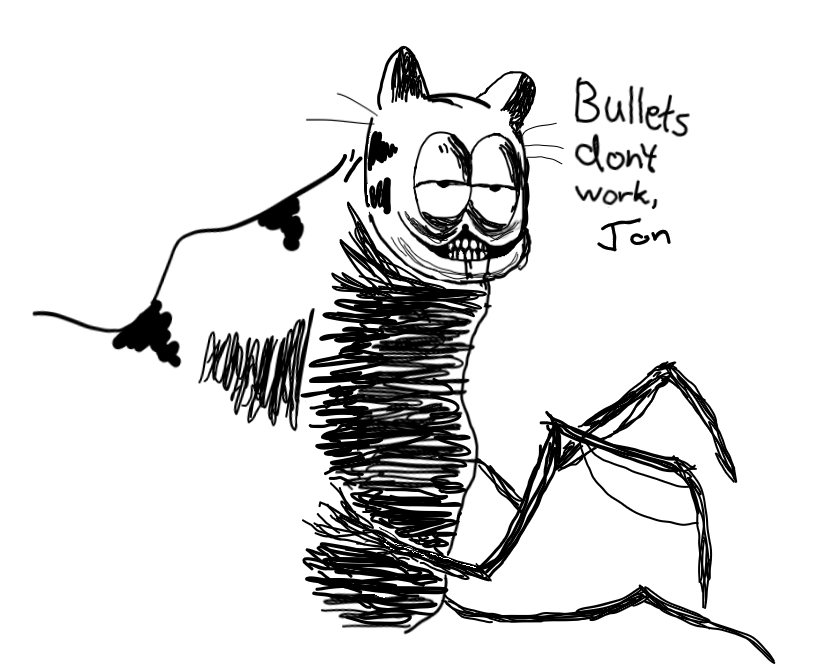
\includegraphics[width=3in]{jon1}
    \caption{Bullets don't work, Jon.}
    \label{fig:Aircraft}
\end{figure}

Characteristics of the aircraft are shown in Table~\ref{table:UASPerformance}.

%Illustrate inserting a table
\begin{table}
	\begin{center}
	\begin{tabular}{|p{6cm}|p{6cm}|}
	\hline
	\textbf{Aircraft Characteristics} & \textbf{Values} \\
	\hline
	Total Weight & 2.917 kg \\
	\hline
	Endurance & $\approx$ 15 minutes \\
	\hline
	Center of Gravity & 17.75 in. aft of aircraft nose\\
	\hline
	\end{tabular}
	\caption{UAS performance specifications.}
	\label{table:UASPerformance}
	\end{center}
\end{table}

The ground control station (GCS) is shown in Figure~\ref{fig:GroundControlStation}.  

\begin{figure}[ht]
	\centering
    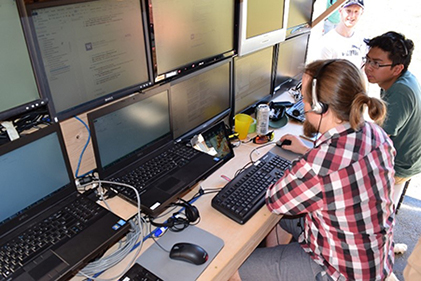
\includegraphics[width=3in]{GroundControlStation}
    \caption{Operators at the GCS.}
    \label{fig:GroundControlStation}
\end{figure}

\subsection{Algorithms}

An example of an equation is given in Eq.~\ref{eqn:KalmanUpdate}.

%Illustrate inserting an equation
\begin{equation}
	K = P_{predicted} H^{T} \Big( H P_{predicted} H^{T}+R\Big) ^{-1}
	\label{eqn:KalmanUpdate}
\end{equation}

%Illustrate breaking the document into several .tex files and then including them together with 'input'
\section{Conclusions}
Here are the conclusions.  Note that this is a separate .tex file which is included into the larger document.

%Illustrate creating a bibliography by referring to an external bibliography file (SampleBibliography.bib).  Note that you must chose a style to determine how the bibliography is presented
\bibliography{SampleBibliography}
\bibliographystyle{aiaa}

\end{document}
